\documentclass[8pt]{extarticle}
\title{}
\author{Avinash Iyer}
\date{}
\usepackage[shortlabels]{enumitem}

%font setup
%
%\usepackage[math]{anttor}

%paper setup
\usepackage{geometry}
\geometry{letterpaper, portrait, margin=1in}
\usepackage{fancyhdr}

\usepackage{blkarray}
\usepackage{nicematrix}
%symbols
\usepackage{amsmath}
\usepackage{mathtools}
\usepackage{amssymb}
\usepackage{hyperref}
\usepackage{gensymb}

\usepackage[T1]{fontenc}
\usepackage[utf8]{inputenc}

%chemistry stuff
\usepackage[version=4]{mhchem}
\usepackage{chemfig}

%plotting
\usepackage{pgfplots}
\usepackage{tikz}

%\usepackage{natbib}

%graphics stuff
\usepackage{graphicx}
\graphicspath{ {./images/} }

%code stuff
%when using minted, make sure to add the -shell-escape flag
%you can use lstlisting if you don't want to use minted
%\usepackage{minted}
%\usemintedstyle{pastie}
%\newminted[javacode]{java}{frame=lines,framesep=2mm,linenos=true,fontsize=\footnotesize,tabsize=3,autogobble,}
%\newminted[cppcode]{cpp}{frame=lines,framesep=2mm,linenos=true,fontsize=\footnotesize,tabsize=3,autogobble,}

\usepackage{listings}
\usepackage{color}
\definecolor{dkgreen}{rgb}{0,0.6,0}
\definecolor{gray}{rgb}{0.5,0.5,0.5}
\definecolor{mauve}{rgb}{0.58,0,0.82}

\lstset{frame=tb,
	language=Java,
	aboveskip=3mm,
	belowskip=3mm,
	showstringspaces=false,
	columns=flexible,
	basicstyle={\small\ttfamily},
	numbers=none,
	numberstyle=\tiny\color{gray},
	keywordstyle=\color{blue},
	commentstyle=\color{dkgreen},
	stringstyle=\color{mauve},
	breaklines=true,
	breakatwhitespace=true,
	tabsize=3
}
% text + color boxes
\usepackage{tcolorbox}
\tcbuselibrary{breakable}
\newtcolorbox{problem}[1]{colback = white, title = {#1}, breakable}
\newtcolorbox{solution}{colback = white, colframe = black!75!white, title = Solution, breakable}
%including PDFs
\usepackage{pdfpages}
\setlength{\parindent}{0pt}

\pagestyle{fancy}
\fancyhf{}
\rhead{Avinash Iyer}
\lhead{Homework solutions up to Midterm 1}
\begin{document}
\section*{1.1}%
\subsection*{Individual}
\begin{problem}{1.1.1}
  Determine which complete bipartite graphs are complete graphs.
\end{problem}
\begin{solution}
  $K_{1,1}$ is the only complete bipartite graph that is complete
\end{solution}
\begin{problem}{1.1.3}
  Using rectangular blocks whose entries are all equal, write down an adjacency matrix for $K_{m,n}$.
\end{problem}
\begin{solution}
  
  \[
    K_{m,n} = \begin{bNiceMatrix}[first-row,first-col]
          & a_1 & a_2 & \cdots & a_m & b_1 & b_2 & \cdots & b_n \\
      a_1 & 0 & 0 & \cdots & 0 & 1 & 1 & \cdots & 1 \\
      a_2 & 0 & 0 & \cdots & 0 & 1 & 1 & \cdots & 1 \\
      \vdots & \vdots & \vdots & \ddots & \vdots & \vdots & \ddots & \vdots \\
      a_m & 0 & 0 & \cdots & 0 & 1 & 1 & \cdots & 1 \\
      b_1 & 1 & 1 & \cdots & 1 & 0 & 0 & \cdots & 0 \\
      b_2 & 1 & 1 & \cdots & 1 & 0 & 0 & \cdots & 0 \\
      \vdots & \vdots & \vdots & \ddots & \vdots & \vdots & \ddots & \vdots \\
      b_n & 1 & 1 & \cdots & 1 & 0 & 0 & \cdots & 0 \\
    \end{bNiceMatrix}
  \]
\end{solution}
\begin{problem}{1.1.5}
    Prove or disprove: If every vertex of a simple graph $G$ has degree 2, then $G$ is a cycle.
\end{problem}
\begin{solution}
  Let $G$ be the following graph:
    \begin{center}
        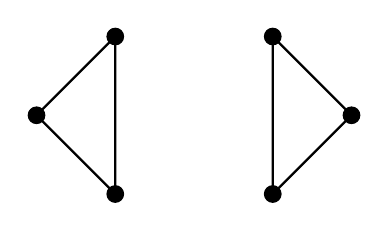
\begin{tikzpicture}
          \draw[fill = black] (1,1) circle (3pt);
          \draw[fill = black] (1,-1) circle (3pt);
          \draw[fill = black] (2,0) circle (3pt);

          \draw[fill = black] (-2,0) circle (3pt);
          \draw[fill = black] (-1,1) circle (3pt);
          \draw[fill = black] (-1,-1) circle (3pt);

        \draw[thick] (1,1) -- (1,-1) -- (2,0) -- (1,1);
        \draw[thick] (-1,1) -- (-1,-1) -- (-2,0) -- (-1,1);
        \end{tikzpicture}
    \end{center}
    Every vertex in $G$ has a degree 2, yet $G$ is not a cycle. 
\end{solution}
\begin{problem}{1.1.8}
    Prove that the 8 vertex graph below decomposes into copies of $K_{1,3}$ and also into copies of $P_4$
  \begin{center}
      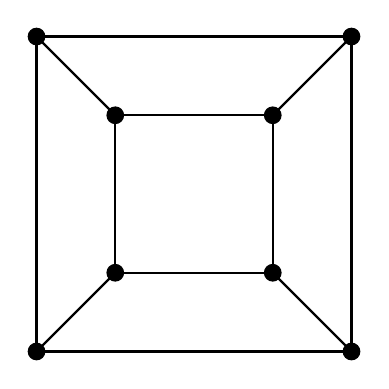
\begin{tikzpicture}
        \draw[fill=black] (1,1) circle (3pt);
        \draw[fill=black] (-1,1) circle (3pt);
        \draw[fill=black] (-1,-1) circle (3pt);
        \draw[fill=black] (1,-1) circle (3pt);

        \draw[fill=black] (2,2) circle (3pt);
        \draw[fill=black] (-2,2) circle (3pt);
        \draw[fill=black] (-2,-2) circle (3pt);
        \draw[fill=black] (2,-2) circle (3pt);
        
        \draw[thick] (1,1) -- (-1,1) -- (-1,-1) -- (1,-1) -- (1,1);
        \draw[thick] (2,2) -- (-2,2) -- (-2,-2) -- (2,-2) -- (2,2);
        \draw[thick] (1,1) -- (2,2);
        \draw[thick] (-1,1) -- (-2,2);
        \draw[thick] (-1,-1) -- (-2,-2);
        \draw[thick] (1,-1) -- (2,-2);
      \end{tikzpicture}
  \end{center} 
\end{problem}
\begin{solution}
    \begin{center}
      \includegraphics[width=10cm]{1_1_8}
    \end{center}
\end{solution}
\begin{problem}{1.1.9}
      Prove that the graph below is isomorphic to the complement of the previous graph
  \begin{center}
      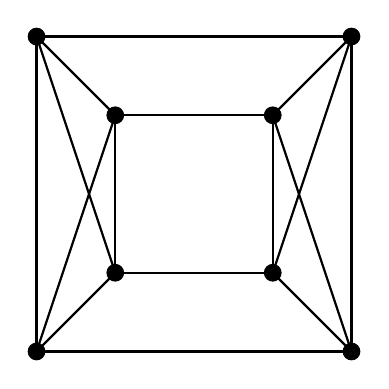
\begin{tikzpicture}
        \draw[fill=black] (1,1) circle (3pt);
        \draw[fill=black] (-1,1) circle (3pt);
        \draw[fill=black] (-1,-1) circle (3pt);
        \draw[fill=black] (1,-1) circle (3pt);

        \draw[fill=black] (2,2) circle (3pt);
        \draw[fill=black] (-2,2) circle (3pt);
        \draw[fill=black] (-2,-2) circle (3pt);
        \draw[fill=black] (2,-2) circle (3pt);
        
        \draw[thick] (1,1) -- (-1,1) -- (-1,-1) -- (1,-1) -- (1,1);
        \draw[thick] (2,2) -- (-2,2) -- (-2,-2) -- (2,-2) -- (2,2);
        \draw[thick] (1,1) -- (2,2);
        \draw[thick] (-1,1) -- (-2,2);
        \draw[thick] (-1,-1) -- (-2,-2);
        \draw[thick] (1,-1) -- (2,-2);
        \draw[thick] (2,2) -- (1,-1);
        \draw[thick] (2,-2) -- (1,1);
        \draw[thick] (-2,2) -- (-1,-1);
        \draw[thick] (-2,-2) -- (-1,1);
      \end{tikzpicture}
  \end{center} 
\end{problem}
\begin{solution}
  \begin{center}
    \includegraphics[width=15cm]{1_1_9}
  \end{center}
\end{solution}
\begin{problem}{1.1.10}
   Prove or disprove: the complement of a simple disconnected graph must be connected.
\end{problem}
\begin{solution}
   Let $G$ be a graph that is disconnected. We want to show that $\forall x,y\in V(G), \exists xz$ path. We can split into two cases.
     \begin{itemize}
       \item Suppose $x\not\leftrightarrow y$ in $G$. Then, in $\overline{G}$, $x\leftrightarrow y$ by the definition of a graph complement.
       \item Suppose $x\leftrightarrow y$ in $G$. Then, since $G$ is disconnected, we know that there must be some $z\in V(G)$ such that there is no $xz$ path. Since there is no $xz$ path, then there is no $yz$ path. In particular, this means $x\not\leftrightarrow z$ and $y\not\leftrightarrow z$ in $G$. Therefore, in $\overline{G}$, we have that $x\leftrightarrow z$ and $y\leftrightarrow z$, meaning there is a path between $x$ and $y$.
     \end{itemize}
\end{solution}
\subsection*{Group}%
\begin{problem}{1.1.13}
    Let $G$ be the graph whose vertex set is the set of $k$-tuples with coordinates $\{0,1\}$, with $x$ adjacent to $y$ if $x$ and $y$ differ by exactly one position. Determine whether $G$ is bipartite.
\end{problem}
\begin{solution}
  $G$ is bipartite --- we can find a bipartition by separating the set into a set of tuples which differ by an even number of positions and a set of tuples which differ by an odd number of positions. Since odd numbers differ from each other by at least $2$ places, and even numbers differ from each other by at least $2$ places, we know that each subset of tuples is not adjacent to each other, but is adjacent to the other set. 
\end{solution}
\begin{problem}{1.1.26}
  Let $G$ be a graph with girth $4$ in which every vertex has degree $k$. Prove that $G$ has at least $2k$ vertices. Determine all such graphs with $2k$ vertices.
\end{problem}
\begin{solution}
  \noindent Suppose $G$ is a graph with girth $4$ with every vertex of degree $k$. Let $v_i\in V(G)$. Then, there must be $k$ vertices which $v_i$ is adjacent to. However, none of these vertices can be adjacent to themselves or $G$ would have girth $3$. Thus, we can form a bipartition such that $v_i$ is in a set of at least $k$ vertices such that each vertex is not adjacent to itself, and each vertex in this set is adjacent to $k$ vertices in a disjoint set where each vertex in this set is not adjacent to any other vertex in this set. Therefore, there are at least $2k$ vertices.\\

  \noindent The graphs with exactly $2k$ vertices are the $K_{n,n}$ complete bipartite graphs.
\end{solution}
\begin{problem}{1.1.27}
    Let $G$ be a graph with girth 5. Prove that if every vertex of $G$ has degree at least $k$, then $G$ has at least $k^2+1$ vertices. For $k=2$ and $k=3$, find one such graph with $k^2+1$ vertices.
\end{problem}
\begin{solution}
  \noindent Let $G$ be a simple graph with girth 5. Suppose that every vertex of $G$ has degree $k$. Let $u\in V(G)$. Then, $u$ has $k$ adjacent vertices, each of which is not adjacent to each other (or else the girth of $G$ would be $3$). Let this set be $N$. The elements of $N$ cannot have any other common neighbors aside from $u$, or else the girth of $G$ would be $4$, meaning each has $k-1$ distinct neighbors. Therefore, the total number of vertices in our graph includes $u$, the elements of $N$ that are the $k$ distinct neighbors of $u$, and the $k(k-1)$ distinct vertices for each vertex in $N$. Therefore, our total is $1 + k + k(k-1) = k^2 + 1$.\\

  \noindent If there were any vertex with degree greater than $k$, then there would be additional vertices beyond the $k^2 + 1$ vertices necessary for a $k$-regular graph.\\

  \noindent For  $k=2$, we have the graph $C_5$ for an example of a graph with $k^2 + 1$ vertices, and for $k=3$ we have the Petersen graph.
\end{solution}
\begin{problem}{1.1.30}
    Let $G$ be a simple graph with adjacency matrix $A$ and incidence matrix $M$. Prove that the degree of $v_i$ is the $i$th diagonal entry of $A^2$ and $MM^T$. What do the entries in position $(i,j)$ of $A^2$ and $MM^T$ say about $G$?
\end{problem}
\begin{solution}
  \noindent Let $A$ be the adjacency matrix for a simple graph $G$. In $A$, every vertex's corresponding row and column are identical, meaning that the entry $A^2_{i,i}$ will be equal to $r_ic_i$ for row $i$ and column $i$ corresponding to $v_i$. Thus, $r_ic_i$ is equal to $|c_i|^2$, which is equal to the sum of the elements of $c_i$, which is equal to the degree of $v_i$.\\

  \noindent Let $M$ be the incidence matrix for a simple graph $G$. In $MM^T$, the diagonal element $MM^T_{i,i}$ will be equal to $r_i r_i^T$, where $r_i$ represents the edge incidence row of $v_i$. This is equal to $\left|r_i^T\right|^2$, which is equal to the sum of the elements of $r_i$, which is equal to the number of edges incident on $v_i$, which is equal to the degree of $v_i$.\\

  \noindent The entry in position $(i,j)$ in both $A^2$ and $MM^T$ shows whether vertices $v_i$ and $v_j$ are adjacent to each other.
\end{solution}
\begin{problem}{1.1.34}
    Decompose the Petersen graph into three connected subgraphs that are pairwise isomorphic. Also decompose it into copies of $P_4$.
\end{problem}
\begin{solution}
  \begin{center}
    \includegraphics[width = 15cm]{1_1_34.pdf}
  \end{center}
\end{solution}
\section*{1.2}%
\subsection*{Individual}%

\end{document}
